% id: 8-06
% book: 100발100중 3-2 기말 · 01 3-2 기말(원의 성질·통계·부록)
% section: 기출 Best
% figure: crop:fig-8-06.png
% answer: ②
% answer_source: 답지(빠른정답)
% variant_level: 0 (원본 전사)
% 이 파일은 build.mjs 가 items.json 에서 만든다. 고칠 때는 items.json 을 고친다.
\smash{\raisebox{1.5mm}{\dmkichul{100발100중 3-2 기말 8쪽 06번}}}
\noindent\begin{minipage}[t]{0.58\linewidth}\vspace{0pt}\raggedright 그림에서 $\seg{AB}$는 원~$\pt{O}$의 지름이고 $\angle\pt{PBA}=62^\circ$일 때, $\angle x$의 크기는?\end{minipage}\hfill\begin{minipage}[t]{0.4\linewidth}\vspace{0pt}\centering 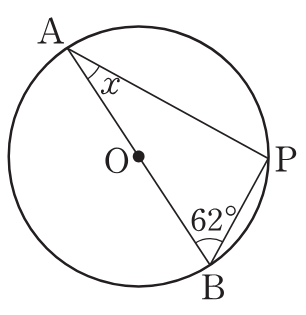
\includegraphics[width=73.2pt]{figures/fig-8-06.png}\end{minipage}\par
\begin{choicesii}{$18^\circ$}{$28^\circ$}{$32^\circ$}{$36^\circ$}{$40^\circ$}\end{choicesii}
